\documentclass[a4paper, 12pt]{article}
%\usepackage[utf8]{inputenc} 
\usepackage[frenchb]{babel}
\usepackage{fullpage}
\usepackage[T1]{fontenc} 
\usepackage{graphicx}  
\usepackage[final]{pdfpages}
\usepackage{amsmath, amssymb,amsthm}
\usepackage{algorithm,algorithmic}
\usepackage{listingsutf8}
\usepackage{lmodern}
\usepackage{tikz}
\usepackage{pgfplots}
\usepackage{fancybox}
%\usepackage{slashbox}
\usepackage{makecell}
\usepackage{array, multirow, tabularx}
\usepackage{xcolor}
\setlength{\parskip}{\bigskipamount}

\newtheorem{mydef}{Définition}
\newtheorem{thm}{Théorème}
\newtheorem{lem}{Lemme}
\newtheorem{cor}{Corollaire}
\newtheorem{prop}{Propriété}

\title{Rapport de Méthodes approchées.}
\author{Dyce William, Loukil Amal, Ouazzani-chahdi Sabrina : \\ M1 IMAGINA--MOCA}
\date{semestre 2 : 2011-2012}

\begin{document} 

\maketitle

\begin{abstract}
  Le présent document consiste en un mémoire au sujet
  d'exercices à la fois théoriques et pratiques sur diverses
  problèmatiques liées à l'étude de méthodes approchées pour la
  résolution de problèmes NP-difficiles. 
\end{abstract}
\vspace{2cm}
\textit{Travelling Salesman Problem :}
\begin{figure}[h!]
\centering
\includegraphics[height = 9cm]{../images/commerce.png}
\end{figure}


\pagebreak

\tableofcontents

\pagebreak

\listoffigures

\listoftables
\pagebreak

\section{Généralités et notations}

Le rapport que nous vous présentons ici reprend notre travail effectué
dans le cadre du projet du cours de méthodes approchées. Celui-ci se
compose d'une partie théorique nous laquelle nous avons résolu divers
exercices traitant de programmation linéaire, d'approximations de
problèmes NP-difficiles, mais aussi de méthodes exactes comme la
programmation dynamique ou les méthodes de branchement (branch and
bound et branch and cut), ainsi que d'une partie pratique. Dans cette
dernière, nous programmons les formules de programmation dynamique
pour trois problèmes classiques (partition, sac à dos, voyageur de
commerce), puis nous nous intéressons plus en détail au cas du
voyageur de commerce avec la programmation de l'algorithme de branch
en bound (après application et comparaison de diverses heuristiques
pour trouver une solution initiale).


On notera en général $PL$ un programme linéaire, et $PLNE$ un
programme linéaire en nombres entiers. 


Nous désignerons également par $TSP$ le problème du voyageur de
commerce.


Rappelons enfin les quelques définitions clés suivantes~:
\begin{mydef}
Les méthodes de branch and bound sont les méthodes dites de séparation
et évaluation.
\end{mydef}

\begin{mydef}
Les méthodes de branch and cut sont les méthodes dites des coupes de
Gomory ou d'algorithmes de coupe.
\end{mydef}

\begin{mydef}
Un problème NP-Complet est un problème de décision pour la résolution duquel on ne
connait pas d'algorithme polynomial. Tous les problèmes de la classe
NP peuvent se rammener à un problème NP-complet via une réduction polynomiale.
\end{mydef}

\begin{mydef}
Un problème NP-Difficile est un problème d'optimisation qui est plus
difficile qu'un problème NP-Complet.
\end{mydef}

\pagebreak

\section{Partie théorique}

\subsection{Programmation linéaire en nombres entiers}

\subsubsection*{Exercice 1}
\paragraph{Question 1}

\begin{itemize}
\item[] a) Le programme linéaire en nombre entier présenté dans
  l'énoncé se justifie de la manière suivante~:
\begin{itemize}
\item $x_j \in \{0,1\}, j=1..n$ car on a le choix binaire entre prendre un
  sommet (donc le compter avec 1), ou ne pas le prendre (ne pas le
  compter avec 0, élément neutre de l'addition). Il y a bien
  évidemment n sommets, d'où l'indexation de 1 à n.
\item $min z = \sum^n _{i=1} x_i$ car on souhaite minimiser le nombre
  de sommets pris.
\item $x_r + x_s \geq 1$ car au moins un sommet doit être pris pour
  couvrir une arête.
\end{itemize}
Ces trois conditions décrivent donc bien le problème de la couverture minimale.
\item[] b) Le cas du triangle est un contre-exemple qui contredit cette
égalité. En effet (cf le dessin ci-dessous) le fait de
choisir l'arête $AC$, par exemple, empêcherait de sélectionner les
autres arêtes (sous peine de violer la contrainte d'égalité) alors
qu'un sommet resterait insaturé. Cette condition doit donc être
élargie à une inégalité.
\begin{figure}[!ht]
\begin{center}
\includegraphics[height=3cm]{../images/triangle.eps}
\end{center}
\caption{Pourquoi on ne peut pas avoir $x_r + x_S = 1$.}
\end{figure}
\item[] c) Montrons par l'absurde que le programme linéaire en nombres
  entiers est une borne inférieure de toute solution optimale.
\begin{proof}
Supposons que pour une instance donnée, on ait une solution optimale
de vertex cover qui soit meilleure que PLNE. Cela veut donc dire que
PLNE garde au au moins un sommet <<~en trop~>>. Or PLNE devrait
minimiser le nombre de sommets et le simplexe est adéquat. Le résultat
est donc absurde et contredit notre hypothèse de départ.
\end{proof}
\item[] d) Nous allons ici montrer de deux manières différentes que la
  relaxation des contraintes d'intégrité implique $x_r \geq
  \frac{1}{2}$ ou $x_s \geq \frac{1}{2}$.
\begin{itemize}
\item Première démonstration.
\begin{proof}
On veut, malgré la relaxation des contraintes d'intégrité, conserver
l'inégalité $x_r + x_s \geq 1$. Ainsi, on a $\neg (x_r + x_s < 1)$
d'où $\neg (x_r < \frac{1}{2} \wedge x_s < \frac{1}{2})$, et donc
($x_r \geq \frac{1}{2} \vee x_s \geq \frac{1}{2}) $ de par la loi de
De Morgan.
\end{proof}
\item Deuxième démonstration.
\begin{proof}
On sait que $A \Rightarrow B \equiv \neg A \vee B$. 
Or, pour respecter l'inégalité $x_r + x_s \geq 1$, on a $(x_r <
\frac{1}{2} \Rightarrow x_s \geq \frac{1}{2})$. On a ainsi $(x_r \geq
\frac{1}{2} \vee x_s \geq \frac{1}{2})$. 
\end{proof}
\end{itemize}
\item[] e) Montrons que l'algorithme 1 conduit à un algorithme
  approché avec une performance relative de de deux. 
\begin{proof}
Soit $C^{*}$ une solution optimale du problème de la couverture de
sommet. Soit $C$ la solution donnée par l'algorithme. 
$x_r=x_s=\frac{1}{2}$. Après la phase d'arrondi $x_r=x_s= 1$. D'où $
OPT = \frac{approche}{2}$.
En effet, on a pour exemple de pire des cas un carré, cf figure
ci-dessous.
\end{proof}

\begin{figure}
\begin{center}
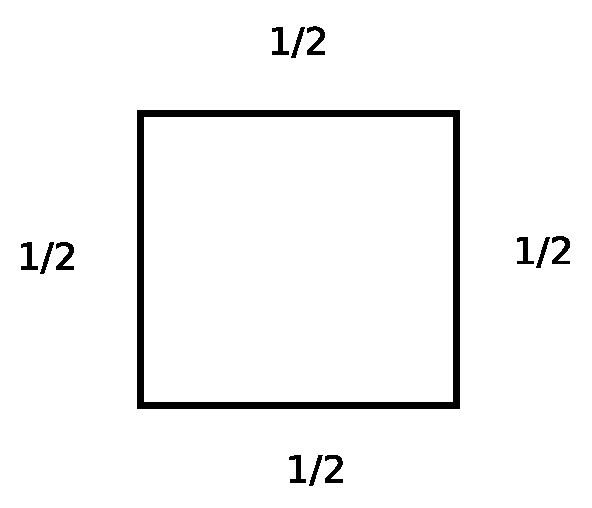
\includegraphics[height=3cm]{../images/carre.eps}
\end{center}
\caption{Pire des cas pour l'algorithme 1}
\end{figure}

\item[] f)
\begin{itemize}
\item i)
Le programme linéaire correspondant à rajouter un poids aux arêtes au
problème du vertex cover est le suivant~:
\begin{equation}
\begin{cases}
min \sum_{i=1}^n w_{i, j}x_i \\
x_r + x_s \geq 1 \\
x_i \in \{ 0, 1 \} \\
\end{cases}
\end{equation}
\item ii)
\begin{equation}
\begin{cases}
min w^Tx \\
A^Tx \geq 1 \\
x_j \in \{0, 1\} \\
\end{cases}
\end{equation}
avec A matrice d'incidence sommets-arêtes.
\item iii) \begin{proof}
$x_i^*\geq \frac{1}{2} \Rightarrow x_i = 1$ \\
$x_i \leq 2x_i^*$ \\
$\Rightarrow C_{PLNE}=\sum x_iw_i \leq (2x_i^*)w_i \leq 2C_{opt}$ \\
\end{proof}
\end{itemize}
\end{itemize}

\paragraph{Question 2}

\begin{itemize}
\item[] a) Montrons que l'algorithme 2 est 2-approché.
\begin{proof}
Soit $C^{*}$ une solution optimale du problème de la couverture sommet et $C$ la solution donnée par l'algorithme. Notons que les arrêtes correspondants aux couples de sommets u et v choisies à chaque itération de l'algorithme correspondent à un couplage maximale $M$. 

Nous avons donc \mbox{$|M| = 2|C|$}. 2 arrêtes de $M$ ne pouvant, par définition d'un couplage, être couverts par un même sommet de $C^{*}$ nous avons forcément \mbox{$|C^{*}| \geq |M|$}

Or \mbox{$|M| = 2|C|$} donc \mbox{$|C^{*}| \geq 2|C|$} d'où \mbox{$\frac{C^{*}}{C} \leq 2$}.

Nous arrivons donc à un taux d'approximation borné par 2.
\end{proof}

\item[] b) Il suffit de prendre $C_4$.
\item[] c) Dans le pire des cas donné à la figure 1, l'algorithme renvoie
  une solution $C$ de taille 8. Or la solution optimale $C^*$ pour cette
  instance est de taille 5. En effet, aucun des sommets de plus haut
  degré n'est inclus dans $C^{*}$. Le choix du sommet de plus haut
  degré n'est donc pas une bonne heuristique. 

En revanche, on peut remarquer que cet algorithme trouve la
  solution optimale sur $C_4$ (qui était le cas limite de l'algorithme 2).
\end{itemize}


\subsubsection*{Exercice 2}
\paragraph{Question 1}

Nous proposons la modélisation suivante en programmation linéaire en
nombres entiers pour le problème de la couverture d'ensembles~:
\begin{equation}
\begin{cases}
min \sum_{j=1}^m w_j s_j\\
\sum_{j=1}^{m} s_{j} \geq 1 \\
s_i \in \{0,1\} \\
\end{cases}
\end{equation}
avec $s_j = 1$ si l'ensemble $S_j$ est choisi, 0 sinon.

Proposition sous forme  d'écriture matricielle, avec M matrice
d'appartenance d'un élément $e_i$ à un ensemble $S_j$~:

\begin{equation}
\begin{cases}
min \sum_{j=1}^m w_j x_j\\
\forall i \in \{1, \dots n \} \sum_{j=1}^{m} M_{ij}x_{j} \geq 1 \\
\forall i \in \{1, \dots n\} x_i \in \{0,1\} \\
\end{cases}
\end{equation}
avec $x_j = 1$ si l'ensemble $S_j$ est choisi, 0 sinon.

\paragraph{Question 2}
 Dans un programme en nombre réels, on a plutôt$ s_j \in [0,1]$. Nous
 proposons donc la procédure d'arrondis suivante sur les $s_j$~:
\begin{itemize}
\item Si $s_j \geq \frac{1}{f}$ alors $s_j = 1$,
\item si $s_j < \frac{1}{f}$ alors $s_j = 0$.
\end{itemize}

\paragraph{Question 3}

La procédure d'arrondie précédente garantie une solution réalisable
car elle respecte toutes les contraintes de la modélisation énoncée à
la question 1.

\begin{proof}
Soit $e$ un élément quelconque de $E$. $e$ appartient à au plus $f$ ensembles donc $\sum\limits_{e \in S_{i}} x_{s} \geqslant 1$. Donc $x_{s} \geqslant \frac{1}{f}$ et donc $e$ est couvert.  
\end{proof}

\paragraph{Question 4}

Montrons que le problème de la couverture d'ensemble possède un
algorithme $f$-approché.

\begin{proof}
Soit $C^*$ une solution optimale pour le problème de la couverture
d'ensemble, soit C la solution renvoyée par un algorithme
$f$-approché.

$C^* \geq  \sum_{i=1}^n w_{e_i}$ car deux éléments peuvent appartenir à un même sous-ensemble.
$C \leq f * \sum_{i=1}^n w_{e_i}$ car un élément appartient a au plus $f$ sous-ensembles \\

On a donc $\frac{C}{C^*} \leq f$.
\end{proof}

\paragraph{Question 5}

Quand $f_i = 2$, $e_i$ appartient à deux sous-ensembles. On retrouve
donc le problème de la couverture d'arêtes (les éléments) par des
sommets (les sous-ensembles) (vertex cover).


\subsubsection*{Exercice 3}
\paragraph{Question 1}Le programme linéaire en nombres entiers qui modélise le
  problème du couplage maximum de poids minimum est le suivant.
  (notons $u_{ij}$ les arêtes du graphe)
Notons que $u_{ij} \in \{0, 1\}$ car on prend une arête ou on ne la
prend pas.

\begin{equation}
\begin{cases}
min \sum w_{ij} u_{ij} \\
\forall x_{ij} \in E ~ \sum u_{i' j'} = 1 \\
 x_{i' j'} \in adj(x_{ij}) \cup \{ x_{ij} \} \\
\end{cases}
\end{equation}

En effet, soit $\{ i, j \}$ une arête qui appartient à un couplage
$M$. Par définition, $\Gamma^{-1}(i) $ et $\Gamma^{+1}(j)$
n'appartiennent pas à $M$.

\paragraph{Question 2}
Les équations des contraintes pour le graphe donné par la figure 2
sont les suivantes~:
\begin{equation}
\begin{cases}
u_{ab}+u_{ac}+u_{ae}=1 \\
u_{ab}+u_{bc}+u_{bf}=1 \\
u_{fb}+u_{fd}+u_{fe}=1 \\
u_{ca}+u_{cb}+u_{cd}=1 \\
u_{dc}+u_{df}+u_{de}=1 \\
u_{ef}+u_{ed}+u_{ea}=1 \\
\end{cases}
\end{equation}

\paragraph{Question 3}
Une solution optimale $z(ILP)$ pour le graphe de la figure 2 est un
couplage de taille 3 et de poids $2.\epsilon + M$ ($= 10,2$ en prenant$\epsilon = \dfrac{1}{10}$ et $M=10$), qui peut par
exemple être $\{
ac, bf, de \}$. 

\paragraph{Question 4}
Le programme relaxé consiste à considérer $0 \leq u_{ij} \leq 1$. \\
Nous avons procédé à la modélisation suivante pour le solveur en ligne
de zweigmedia, en prenant $\epsilon = \dfrac{1}{10}$ et $M=10$~:
\begin{lstlisting}
Minimize p = (1/10)uab + (1/10)uac + (1/10)ubc + 10ubf + 10ucd +
(1/10)udf + (1/10)ude + (1/10)ufe + 10uae subject to


uab + uac + uae = 1 
uab + ubc + ubf = 1 
ubf + udf + ufe = 1 
uac + ubc + ucd = 1 
ucd + udf + ude = 1
ufe + ude + uae = 1 

uab >= 0
ubc >= 0
uac >= 0
ubf >= 0
ucd >= 0
uae >= 0
ude >= 0
udf >= 0
ufe >= 0

uab <= 1
ubc <= 1
uac <= 1
ubf <= 1
ucd <= 1
uae <= 1
ude <= 1
udf <= 1
ufe <= 1
\end{lstlisting}

Ce qui nous donne la solution relaxée suivante~:
\begin{lstlisting}
Optimal Solution: p = 0.3; uab = 0.5, uac = 0.5, ubc = 0.5, ubf = 0,
ucd = 0, udf = 0.5, ude = 0.5, ufe = 0.5, uae = 0
\end{lstlisting}
On a donc un couplage de taille $6$ pour un poids de $0,3$.

\paragraph{Question 5}
On remarque une grande différence entre la solution relaxée et la
solution optimale du problème initial, laissant à penser à une
mauvaise modélisation.


La formulation initialement proposée n'est pas pertinente car elle ne
couvre pas tous les cas. Le fait de répondre au problème du couplage
maximum de poids minimum vérifie nos équations, mais la réciproque
n'est pas vrai. On peut ainsi considérer le contre-exemple suivant
dans lequel le couplage obtenu n'est pas maximum~:
\begin{figure}[!ht]
\begin{center}
\includegraphics[height=2cm]{../images/exo3.eps}
\end{center}
\caption{Contre exemple pour la formulation proposée à l'exercice 3}
\end{figure}


\subsection{Problèmes appartenant à la classe APX}

\subsubsection*{Exercice 4}
\paragraph{Question 1}
La complexité est de $O(m(n+m))=O(n^4)$ car~:
\begin{itemize}
\item La taille de la coupe augmente d'un sommet à chaque tour, donc
il nous faut $m$ étapes pour trouver la coupe maximum.
\item À chaque tour, on rajoute un également toutes les arêtes
incidentes au sommet rajouté.
\end{itemize}

\paragraph{Question 2}
Montrons que le taux d'approximation est de 2~:
\begin{proof}Soit $(Y_1,Y_2)$ la coupe approximatif. Supposons pour $\Gamma(x)$ l'ensemble des sommets voisins d'un sommet x~:

$\exists x \in Y_1 \text{ | } \Gamma(x) \cap Y_1 > \Gamma(x) \cap Y_2$

Dans un tel cas le déplacement du sommet x dans $Y_2$ augmenterai la valeur de la coupe, donc l'algorithme approché ne l'aurait jamais gardé dans $Y_1$. Notre supposition est donc absurde. Nous avions au contraire~:

$\forall x \in Y_1 \text{ | } \Gamma(x) \cap Y_1 \leq \Gamma(x) \cap Y_2$

Le même raisonnement tient pour les sommets de $Y_2$. Or la somme des degrés est égale à $2|E|$ donc~:

\begin{eqnarray*}
2|E| &=& \Sigma_{x \in Y_1}|\Gamma(x)|  + \Sigma_{x' \in Y_2}|\Gamma(x')| \\
	 &=& \Sigma_{x \in Y_1}[|(\Gamma(x)\cap{} Y_1)|\cup|(\Gamma(x)\cap{}Y_2)|] +
	 	 \Sigma_{x' \in Y_2}[|(\Gamma(x')\cap{} Y_1)|\cup|(\Gamma(x')\cap{}Y_2)|] \\
	 &=& \Sigma_{(x,x') \in (Y_1,Y_2)} +
	 	 \Sigma_{(y,y') \in (Y_2,Y_1)} + 
	 	 \Sigma_{(z,z') \in (Y_1,Y_1)} +
	 	 \Sigma_{(t,t') \in (Y_2,Y_2)} 
\end{eqnarray*}

Or $\Sigma_{(x,x') \in (Y_1,Y_2)} \geq \Sigma_{(z,z') \in (Y_1,Y_1)}$ et $\Sigma_{(y,y') \in (Y_2,Y_1)} \geq \Sigma_{(t,t') \in (Y_2,Y_2)}$ nous avons~:

\begin{eqnarray*}
\Sigma_{(x,x') \in (Y_1,Y_2)} + \Sigma_{(y,y') \in (Y_2,Y_1)} &\geq& |E| \\
\Rightarrow |(Y_1, Y_2)| &\geq& \frac{|E|}{2}
\end{eqnarray*}

Globalement au moins la moité des arrêtes doivent donc traverser la coupe approximatif. De plus la coupe optimale est évidement borné par $|E|$, donc $\frac{(Y_1,Y_2)}{(Y_1,Y_2)^*} \geq \frac{|E|}{2|E|}$, soit $\frac{(Y_1,Y_2)^*}{(Y_1,Y_2)} \geq 2$, \emph{quod erat demonstrandum}.
\end{proof}

\paragraph{Question 3}

Prenons le graphe figure \ref{coupe_max_instance}. La coupe optimale (figure \ref{coupe_max_opt}) traverse chacun des 15 arrêtes, il suffit donc de montrer que la coupe approximatif n'en traverse que 7. 

\begin{figure}[ht]
% LEFT-HAND SIDE
\begin{minipage}[b]{0.5\linewidth}
\centering
\centering
\includegraphics[width=0.4\textwidth]{../images/exo4.eps}
\caption{Instance coupe maximum.}
\label{coupe_max_instance}
\end{minipage}
% RIGHT-HAND SIDE
\hspace{0.5cm}
\begin{minipage}[b]{0.4\linewidth}
\centering
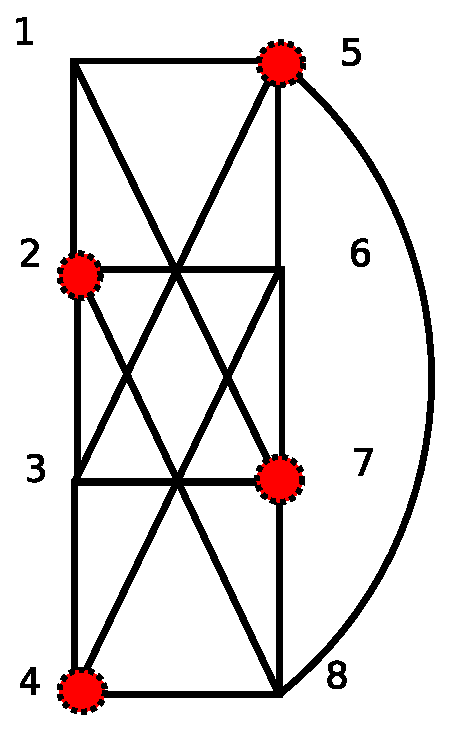
\includegraphics[width=0.5\textwidth]{../images/exo4_opt.eps}
\caption{Coupe optimale.}
\label{coupe_max_opt}
\end{minipage}
\end{figure}

Pour l'instant nous n'avions pas réussis à expliciter une telle coupe. Pourtant l'algorithme n'est pas optimale~: il sera bloqué sur $P_4$ avec une coupe de valeur 2 s'il avait la mal chance de prendre les deux extrémités. Pour ceci n'est une erreur d'approximation de $frac{2}{3}$.

Peut être que la taux d'approximation de cette algorithme est en fait plus basse que 2\dots


\subsection{Constructions de PTAS}

\subsubsection*{Exercice 5}
Amal
\paragraph{Question 1}

\paragraph{Question 2}

\begin{itemize}
\item a)
\item b)
\item c)
\end{itemize}

\paragraph{Question 3}

La complexité de l'algorithme 

\subsubsection*{Exercice 6}
\paragraph{Question 1}
\begin{itemize}
\item a) $nlogn+n = O(nlogn)$
\item b) Si $j = 1$ alors $cost(T) + w_{2} \geqslant B$ et donc $cost(T) \geqslant \frac{B}{2}$.\\
Si $j \geqslant 2$ alors $\sum_{i=1}^{j} W_{j} + W_{j+1} \geqslant B$, c'est à dire $\sum_{i=1}^{j} \geqslant W_{j+1}$ et donc $cost(T) > \frac{B}{2}$.
\item c)  $s^{*} \geqslant B$ et $S \geqslant \frac{B}{2}$\\
$\frac{1}{S} \leqslant \frac{2}{B}$ et donc $\frac{S^{*}}{S} \leqslant 2$.
\end{itemize}

\paragraph{Question 2}
\begin{itemize}
\item a) L'algorithme $2$ admet une complexité de $O(n^{k+1})$ car ~:
\begin{itemize}
\item pour étendre $S$ à $S^*$ on a un coût de $O(nlogn)$~;
\item les ensembles $S$ de taille maximale $k$ sont créés avec un coût
de k parmi n, c'est à dire en $O(n^k)$.
\end{itemize}
\item b)
\begin{itemize}
\item i) Si $p \leq k$ alors on est à l'optimal (puisqu'on s'est
arrêtés avant le $k$).
\item ii)
\begin{itemize}
\item A) Si $P^*=M$ alors c'est que la solution est optimale.
\item B) Montrons que $\exists i_q > i_k \geq k$ tel que
$cost(P^*)+w_iq > b \geq cost(M)$.
\begin{proof}
Par définition de l'optimalité, on a $cost(M) \leq b$. $k$ est
l'indice associé à la solution optimale, par définition de la
notation. \\
$cost(P^*) \leq b$ mais $cost(P^*) + w_{i_q} > b$ car sinon $w_{i_q}$
aurait déjà fait partie de la solution (on a $i_q > i_k$). 
\end{proof}
\item C) Montrons que $w_{i_q} \leq \frac{cost(M)}{k+1}$.
\begin{proof}
Si ce n'était pas le cas, on pourrait rajouter $w_{i_q}$ dans
notre solution. En effet, la fraction $\frac{cost(M)}{k+1}$ est
l'espace qu'il reste jusqu'à la solution optimale en prenant un objet
de plus que ce qu'on a pris jusqu'à présent.
\end{proof}
\item D) Évaluons le ratio $R(I, \epsilon)
= \frac{cost(M)}{cost(P^*)}$. \\
TODO


\end{itemize}
\end{itemize}
\end{itemize}


\subsection{Utilisation de méthodes exactes}

\subsubsection*{Exercice 7}
\paragraph{Sur le problème de la partition}

\begin{itemize}
\item a) La condition nécessaire sur la somme des poids des $n$ objets
  est la suivante~: on veut $\sum_{a \in A'} p(a)= \sum_{a \in A
    \backslash A'}p(a)$
\item b) 
\begin{itemize}
\item i) La formule qui lie les lignes $i$, $i-1$ et $p(a_i)$ est $A_i
  := A_{i-1} \bigcup A_{i, p(a_i)} \bigcup A_{i-1}+p(a_i)$ avec
  $A_{i-1}+p(a_i) \leq P$.
\item ii) TODO
\item iii) Nous proposons les deux algorithmes ci-dessous.
\begin{algorithm}[t]
\caption{Algorithme général}
\label{algoexo7}
\begin{algorithmic}[1]
\STATE $P_1 := \emptyset $,  $P_1 := \emptyset $
\FOR{$i=1 \to n$}
\WHILE{$P_1 < P$ et $P_2 < P$}
\STATE remplir $A_i$ en utilisant la formule présentée avant
\STATE faire Test
\IF {$A(i,j) == 1$}
\STATE $A(i,j):=0$
\ENDIF
\ENDWHILE
\ENDFOR
\end{algorithmic}
\end{algorithm}

\begin{algorithm}[t]
\caption{Test}
\label{algoexo7test}
\begin{algorithmic}[1]
\FOR{$j=0 \to P$}
\IF{$A(i,j) == 1$ et $P_{1}+j \leq P$}
\STATE $P_1 := P_1 \bigcup j$
\ELSE
\STATE $P_2 := P_2 \bigcup j$
\ENDIF
\ENDFOR
\end{algorithmic}
\end{algorithm}
\end{itemize}

\item c) La complexité est donc $O(n\times P)$.
\item d) Nous proposons les traces suivantes pour nos algorithmes~:
\begin{itemize}
\item La première trace que nous proposons est réalisée à partir des
  données fournies dans l'énoncé. Ici, $P=16$. On obtient ainsi $P_1 := \{ 0, 5, 9,
  2, 0\}$, $P_2 := \{ 0, 0, 3, 8, 5\}$.
\item Prenons désormais $P(a_1)=2$, $P(a_2)=4$, $P(a_3)=3$,
  $P(a_4)=1$. Ici, $P=5$. On obtient ainsi  $P_1 := \{ 0, 2, 3\}$,
  $P_2 := \{ 0, 4, 1\}$.
\item Prenons désormais $P(a_1)=2$, $P(a_2)=4$, $P(a_3)=3$,
  $P(a_4)=6$. Il n'est dans cet exemple pas possible de partager en
  deux sous-ensembles de même poids nos objets. Soit P n'existe pas et
  notre algorithme ne pourra être lancé. Soit P existe et l'algorithme
  donnera le résultat le plus proche possible pour $P_1$, et remplira
  $P_2$ avec tous les objets <<~en trop~>>.
\end{itemize}
\end{itemize}

\paragraph{Le problème du sac à dos}
\begin{itemize}
\item a) Nous justifions les formules proposées en énonçant que l'on
  prend le maximum des $x_ju_j$ pour $j$ de 1 à $k-1$ en enlevant le
  poids de l'objet $x_k$, et l'on rajoute à $x_ju_j$ l'utilité de
  l'objet en cours.
\item b) TODO
\item c) TODO
\end{itemize}



\subsubsection*{Exercice 8}
\paragraph{Question 1}

\begin{itemize}
\item Pour le premier produit, on doit effectuer $P_{k-1}.P_k.P_{k+1}
  + P_{k-2}.P_{k-1}.P_{k+1} + \dots + P_2.P_3.P_{k+1} +
  P_1.P_2.P_{k+1}$ opérations. Donc $O(k^4)$.
\item Pour le parenthésage symétrique, on doit effectuer $P_1.P_2.P_3
  + P_1.P_3.P_4 + P_1.P_4.P_5 + \dots + P_1.P_{k-1}.P_{k} +
  P_1.P_k+P_{k+1}$ opérations. Donc $O(k^3)$.
\end{itemize}

On remarque que le \textit{coefficient} le plus au bout de la matrice
la plus imbriquée (càd $p_{k+1}$ pour le premier produit, et $P_1$
pour le second) est \textit{reporté} à chaque \textit{séquence} de
calcul, et que l'on peut donc factoriser le calcul global par ce
terme. Par conséquent, selon la valeur du terme ainsi répété en
fonction du parenthésage choisi, le nombre d'opérations pour un même
produit de matrices peut énormément varier.

\paragraph{Question 2}

Montrons que le nombre $c(k)$ de parenthésages possibles d'un produit
de $k$ matrices vérifie $\sum_{i=1}^{k-1}c(i).c(k-i)$ en posant
$c(1)=1$. Procédons par récurrence.

\begin{proof}
\begin{itemize}
\item Si l'on multiplie deux matrices, il est clair de voir que nous
  n'avons qu'un seul parenthésage possible. Si l'on applique la
  formule, alors $c(2) = c(1).c(2-1) = c(1).c(1) = 1$. La propriété
  est donc vérifiée pour deux matrices.
\item Supposons désormais que la propriété $c(k) =
  \sum_{i=1}^{k-1}c(i).c(k-i)$ soit vérifiée pour $k$ matrices, et
  montrons qu'elle l'est alors aussi pour $k+1$ matrices. Le fait de
  rajouter une matrice implique de rajouter un certain nombre de
  possibilités de parenthésages possibles. Étudions les~: on rajoute
  autant de parenthésages que de parenthésages existant (une
  parenthèse de plus pour englober ce qui existe déjà) pour chaque
  possibilité de parenthésage. On a donc, $c(k+1)
  =\sum_{i=1}^{k-1}c(i).c(k-i)+c(k).c(k+1-i)= \sum_{i=1}^{k}c(i).c(k+1-i)$.
\end{itemize}
\end{proof}

\paragraph{Question 3}

Afin d'appliquer les principes de la programmation dynamique pour ce
problème (trouver $m_{1,k}$ le coût minimum du produit $M_{1k}$ ainsi
que le parenthésage correspondant), nous décomposons le produit en
deux sous-produits (que l'on peut calculer par récurrence) dont nous
sommons les coûts et auquel nous rajoutons le coût de la
mutliplication des deux matrices ainsi engendrées.

\begin{equation}
\begin{cases}
m_{i,j} = \min \{(m_{i,p}+m_{p+1,j}) + (i \times p+1 \times j+1) \} \\
i \leq p \leq j \\
\end{cases}
\end{equation}

On obtient le parenthésage correspondant à chaque bloc en retenant les
$p$ (une parenthèse à la fin de chaque $p$ et au début de chaque $p+1$).

\paragraph{Question 4}

On a $M_{15} = M_1.M_2.\dots M_5$. \\

On propose donc le tableau suivant pour calculer $m_{1,5}$~:
\begin{center}
\begin{tabular}{|l|c|c|c|c|c|}
\hline  $i$ $\diagdown$ $k$ & $1$  & $2$ & $3$ & $4$ & $5$ \\
\hline $1$ & $1$ & $0$ & $0$ & $0$ & $0$ \\
\hline $2$ & $0$ & $1$ & $0$ & $0$ & $0$ \\
\hline $3$ & $0$ & $0$ & $1$ & $0$ & $0$ \\
\hline $4$ & $0$ & $0$ & $0$ & $1$ & $0$ \\
\hline $5$ & $0$ & $0$ & $0$ & $0$ & $1$ \\
\hline
\end{tabular}
\end{center}

TODO



%\subsection{Méthode Primal-Dual}

%\subsubsection*{Exercice 9}
%\input{ex9.tex}

\subsection{Borne de non-approximation}

\subsubsection*{Exercice 10}
\paragraph{Question 1}

Le problème de bin packing est le problème de trouver un rangement
valide pour tous nos articles, qui minimise le nombre de boîtes
utilisées (avec, bien sûr, la contrainte qu'un objet n'appartienne
qu'à une seule boîte, d'où la troisième ligne de la modélisation
proposée).  On l'exprime de la manière suivante~:
\begin{equation}
\begin{cases}
min \sum_{j=1}^{n}y_j \\
\sum_{i=2}^{n} c_ix_{ij} \leq C_{y_j}, j = 1, \dots, n \\
\sum_{j=1}^{n}x_{ij}=1, i=1, \dots, n \\
x_{i,j} \in \{ 0,1 \} \\
y_j \in \{ 0,1 \} \\
\end{cases}
\end{equation}
Avec $y_j = 1$ si la boîte $j$ est utilisée, 0 sinon. \\
Avec $x_{ij} = 1 $ si article $i$ est rangé dans la boîte $j$, 0
sinon. \\
Avec $c_i$ taille de l'article $i$ et C la taille d'une boîte.


\paragraph{Question 2}
\begin{itemize}
\item a) $B = 32$, $P(a_1') = \frac{5 \times 2}{32} = \frac{10}{32}$,
  $P(a_2') = \frac{9}{16}$, $P(a_3')=\frac{6}{32}$,
  $P(a_4')=\frac{1}{2}$, $P(a_5')=\frac{4}{32}$, $P(a_6')=\frac{10}{32}$.
\item b) $B = 180$, $P(a_1') = \frac{154}{180}$,
  $P(a_2') = \frac{82}{180}$, $P(a_3')=\frac{6}{180}$,
  $P(a_4')=\frac{60}{180}$, $P(a_5')=\frac{34}{180}$, $P(a_6')=\frac{24}{180}$.
\end{itemize}

\paragraph{Question 3}
\begin{itemize}
\item Quand nous avons une instance positive, alors nous avons pour le problème Bin Packing une partition de l'ensemble d'objets en deux sous ensembles dont le poids égale à $\frac{B^{*}}{2}$. Donc, la valeur optimale pour le problème Bin Packing $m^{*} = 2$. 
\item Quand nous avons une instance négative, alors nous avons forcément un objet dont le poids dépasse $\frac{B}{2}$ et on ne nous pouvons pas le mettre ni dans la première boîte ni dans la deuxième. Donc, on doit rajouter une nouvelle boîte, d'où $m^{*} = 3$.
\end{itemize}
\paragraph{Question 4}
Nous avons un algorithme polynomial pour le problème de Bin Packing. Donc, on peut décider en temps polynomial pour le problème partition, or ce problème est NP-complet. Donc, le problème Bin Packing est non ($\frac{3}{2} - \epsilon $)--approché.




\subsubsection*{Exercice 11}
\paragraph{Question 1}

Les deux problèmes considérés sont NP-complets. Plus exactement, la
coloration de sommet est un problème non-APX tandis que la coloration
d'arêtes est un problème APX. 

\paragraph{Question 2~:}
\begin{itemize}
\item Si $OPT(I) \leq 3$ alors on a \\
$\frac{A(I)}{OPT(I)} < \frac{4}{3}$ \\
d'où $A(I) < 4$.
\item Si $OPT(I) \geq 4$ alors on a \\
$\frac{A(I)}{OPT(I)} < \frac{4}{3}$ \\
d'où $A(I) \geq 3$.
\end{itemize}

\paragraph{Question 3~:}

\begin{proof}
Le problème de 3--coloration est NP-complet. Or, à partir de la
question 2, on peut décider si 3 couleur suffisent pour colorier les
sommets ou les arêtes de notre graphe. Donc il est absurde de supposer
qu'il existe un algorithme avec une performance relative strictement
inférieure à $\frac{4}{3}$.
\end{proof}

\subsection{Comparaison de méthodes}




\subsubsection*{Exercice 12}
\paragraph{Question 1}

Vous trouverez sur le graphique ci-dessous une représentation du
polytope associé aux équations de $PL_0$ (aire située à la fois sous la courbe
bleue et sous la courbe rouge).

\begin{figure}[h!]
\centering
\begin{tikzpicture}[scale=1.2]
    \begin{axis}[title=PL, xlabel=x1, ylabel=x2]
      \addplot
        table[col sep=comma]{equ1.csv};
        \addplot
        table[col sep=comma]{equ2.csv};
        \addplot
        table[col sep=comma]{abs.csv};
        \addplot
        table[col sep=comma]{ord.csv};
        \legend{contrainte1, contrainte2}
    \end{axis}
\end{tikzpicture}
\caption{Polytope exercice 12}
\end{figure}

\paragraph{Question 2}
De manière graphique, on trouve environ $x_1 = 1.5$, $x_2 = 3$, $z = 6$.

\paragraph{Question 3}

Résolution du problème donné par la méthode du simplexe.

\begin{table}[h!]	
\centering
	\begin{tabular}{|c|c|c|c|c|c|}
	\hline
      & c & 2 & 1 & 0 & 0 \\ 
      \cline{2-6}
       &  & $x_{1}$ & $x_{2}$  & $x_{3}$  & $x_{4}$ \\
       \hline
   0 & $x_{3}$  $=$ 17 & 2 & 5 & 1 & 0 \\
      \hline
	0 & $x_{4}$ $=$ 10  & 3 & 2 & 0 & 1 \\
	  \hline
	 & Z($x$)$=$ 0 & -2 & -1 & 0 & 0\\
	  \hline
	\end{tabular}
\caption {Tableau 1 du simplex}	
\centering
	\begin{tabular}{|c|c|c|c|c|c|}
	\hline
      & c & 2 & 1 & 0 & 0 \\ 
      \cline{2-6}
       &  & $x_{1}$ & $x_{2}$  & $x_{3}$  & $x_{4}$ \\
       \hline
   0 & $x_{3}$  $=$ $\frac{31}{3}$ & 0 & $\frac{11}{3}$ & 1 & $\frac{-2}{3}$ \\
      \hline
	2 & $x_{1}$ $=$ $\frac{10}{3}$  & 1 & $\frac{2}{3}$ & 0 & $\frac{1}{3}$ \\
	  \hline
	 & Z($x$)$=$ $\frac{20}{3}$ & 0 & $\frac{1}{3}$ & 0 & $\frac{2}{3}$\\
	  \hline
	\end{tabular}
\caption {Tableau 2 du simplex}
\end{table}



\paragraph{Question 4, a) Branch and Bound}
\begin{itemize}
\item Nous utilisons la solution initiale suivante~:
\begin{equation}
\begin{cases}
x_1 = \frac{10}{3} \\
x_2 = 0 \\
x_3 = \frac{31}{3} \\
x_4 = 0 \\
z(x) = \frac{20}{3} \\
\end{cases}
\end{equation}
\item Nous procédons ensuite à la troncature suivante pour obtenir la
  borne inférieure de notre programme en nombres entiers.
\begin{equation}
\begin{cases}
x_1 = 3 \\
x_2 = 0 \\
z(x) = 2 \times 3 + 0 = 6 \\
\end{cases}
\end{equation}
\item Effectuons désormais un branchement sur $x_1$.
\end{itemize}
\vspace{0.5cm}
 \includegraphics[height=60mm]{../images/branchAndBound.eps}
\paragraph{Question 4, b) Branch and Cut}

Vous trouvez ci dessous les différents étapes des tableaux de la
méthode de Branch and Cut. \\
Les étapes intermédiaires sont les suivantes~:
\begin{itemize}
\item on commence par reprendre les résultats de la question
  concernant la résolution par le simplexe, puis l'on fixe la deuxième
  ligne, d'où $i = 2$.
\item $x_2$ et $x_4$ sont les variables qui ne sont pas en base. On
  peut donc écrire $\frac{2}{3} x_2 + \frac{1}{3} x_4 \geq
  \frac{1}{3}$.
\item Graphiquement, cela correspond à $x_1 \leq 3$ car on a 
\begin{equation}
\begin{cases}
2x_1 + 5x_2 + x_3  = 17 \\
3x_1 + 2x_2 + x_4  = 10 \\
\end{cases}
\\
\Rightarrow x_4  = 10 - 3x_1 - 2x_2 
\end{equation}
Ainsi, en remplaçant $x_4$ dans l'équation de l'item précédent, on a
\\
$\frac{2}{3}x_2 + \frac{1}{3}(10-3x_1-2x_2) \geq \frac{1}{3}$ \\
$\frac{2}{3}x_2 + \frac{10}{3} - x_1 - \frac{2}{3}x_2 \geq
\frac{1}{3}$ \\
$\frac{10}{3} - x_1 \geq \frac{1}{3}$ \\
$-x_1 \geq \frac{-9}{3} = -3$ \\
$\Rightarrow x_1 \leq 3$.
\item On rajoute la nouvelle contrainte obtenue dans notre tableau du
  simplexe, que nous résolvons alors par la méthode à deux phases.
\end{itemize}

\begin{table}[h!]	
\centering
	\begin{tabular}{|c|c|c|c|c|c|c|c|}
	\hline
      & c & 0 & 0 & 0 & 0 & 0 & -1 \\ 
      \cline{2-8}
       &  & $x_{1}$ & $x_{2}$  & $x_{3}$  & $x_{4}$ & $x_{5}$ & $y$ \\
       \hline
   0 & $x_{3}$  $=$ $\frac{31}{3}$ & 0 & $\frac{11}{3}$ & 1 & $\frac{-2}{3}$ & 0 & 0 \\
      \hline
	0 & $x_{1}$ $=$ $\frac{10}{3}$  & 1 & $\frac{2}{3}$ & 0 & $\frac{1}{3}$ & 0 & 0 \\
	  \hline
	  -1 & $y$ $=$ $\frac{1}{3}$  & 0 & $\frac{2}{3}$ & 0 & $\frac{1}{3}$ & -1 & 1 \\
	    \hline
	 $\frac{-1}{3}$ & Z($x$)$=$ 0 & 0 & $\frac{-2}{3}$ & 0 & $\frac{-1}{3}$ & 1 & 0\\
	  \hline
	\end{tabular}
\caption {Tableau 1 des coupes de Gomory}
\end{table}
\begin{table}[h!]	
\centering
	\begin{tabular}{|c|c|c|c|c|c|c|}
	\hline
      & c & 2 & 1 & 0 & 0 & 0 \\ 
      \cline{2-7}
       &  & $x_{1}$ & $x_{2}$  & $x_{3}$  & $x_{4}$ & $x_{5}$ \\
       \hline
   0 & $x_{3}$  $=$ $\frac{31}{3}$ & 0 & $\frac{11}{3}$ & 1 & $\frac{-2}{3}$ & 0 \\
      \hline
	2 & $x_{1}$ $=$ $\frac{10}{3}$  & 1 & $\frac{2}{3}$ & 0 & $\frac{1}{3}$ & 0 \\
	  \hline
	0 & $y$ $=$ $\frac{1}{3}$  & 0 & $\frac{2}{3}$ & 0 & $\frac{1}{3}$ & -1 \\
	  \hline
	 & Z($x$)$=$ $\frac{20}{3}$ & 0 & $\frac{-2}{3}$ & 0 & $\frac{-1}{3}$ & 1\\
	  \hline
	\end{tabular}
\caption {Tableau 1 de la méthode à deux phases}
\end{table}
\begin{table}[h!]	
\centering
	\begin{tabular}{|c|c|c|c|c|c|c|}
	\hline
      & c & 2 & 1 & 0 & 0 & 0 \\ 
      \cline{2-7}
       &  & $x_{1}$ & $x_{2}$  & $x_{3}$  & $x_{4}$ & $x_{5}$ \\
       \hline
   0 & $x_{3}$  $=$ $\frac{17}{2}$ & 0 & 0 & 1 & $\frac{-15}{6}$ & $\frac{11}{2}$ \\
      \hline
	2 & $x_{1}$ $=$ 3 & 1 & 0 & 0 & 0 & 1 \\
	  \hline
	1 & $x_{2}$ $=$ $\frac{1}{2}$  & 0 & 1 & 0 & $\frac{1}{2}$ & $\frac{-3}{2}$\\
	  \hline
	 & Z($x$)$=$ $\frac{13}{2}$ & 0 & 0 & 0 & $\frac{1}{2}$ & $\frac{1}{2}$\\
	  \hline
	\end{tabular}
\caption {Tableau 2 de la méthode à deux phases}
\end{table}
On fixe $i = 3$, donc on a $\frac{1}{2} = x_{2} + \frac{1}{2} x_{4} - \frac{3}{2} x_{5}$.(1)\\
On exprime la contrainte en fonction des variables hors base, on obtient $\frac{1}{2} x_{4} + \frac{1}{2} x_{5} \geqslant \frac{1}{2}$ (2). Donc maintenant, on exprime cette contrainte en fonction de $x_{1}$ et $x_{2}$~:
\begin{itemize}
\item $3 = x_{1} + x_{5} \Longrightarrow x_{5} = 3 - x_{1}$ (3)
\item Remplaçons (3) dans (1), on obtient $x_{4} = 1 - 2x_{2} + 9 - 3x_{1}$
\item Remplaçons $x_{4}$ et $x_{5}$ par leur valeur dans (2), on obtient $\frac{1}{2}(1 - 2x_{2} + 9 - 3x_{1}) + \frac{1}{2} (3 - x_{1}) \geqslant \frac{1}{2} \Longrightarrow x_{2} + 2x_{1} \leqslant 6$ 
\end{itemize}
Ajoutons la contrainte de (2) au programme linéaire initial: on obtient $-y_{1} = \frac{1}{2}x_{4} + \frac{1}{2}x_{5} - x_{6} - \frac{1}{2}$. Résolvons, ainsi, le problème par la méthode deux phases.\\
\begin{table}
\centering
\begin{tabular}{|c|c|c|c|c|c|c|c|c|}
	\hline
      & c & 0 & 0 & 0 & 0 & 0 & 0 & -1 \\ 
      \cline{2-9}
       &  & $x_{1}$ & $x_{2}$  & $x_{3}$  & $x_{4}$ & $x_{5}$ & $x_{6}$ & $y_{1}$ \\
       \hline
   0 & $x_{3}$  $=$ $\frac{17}{2}$ & 0 & 0 & 1 & $\frac{-15}{6}$ & $\frac{11}{2}$ & 0 & 0 \\
      \hline
	0 & $x_{1}$ $=$ 3 & 1 & 0 & 0 & 0 & 1 & 0 & 0 \\
	  \hline
	0 & $x_{2}$ $=$ $\frac{1}{2}$  & 0 & 1 & 0 & $\frac{1}{2}$ & $\frac{-3}{2}$ & 0 & 0\\
	  \hline
	-1 & $y_{1}$ $=$ $\frac{1}{2}$  & 0 & 0 & 0 & $\frac{1}{2}$ & $\frac{1}{2}$ & -1 & 1\\
	  \hline
	 & $\frac{-1}{2}$ & 0 & 0 & 0 & $\frac{-1}{2}$ & $\frac{-1}{2}$ & 1 & 0\\
	  \hline
	\end{tabular}
\caption{Tableau 3 de la méthode à deux phases}
\end{table}
Donc la valeur qui sort de la base est $y_{1}$ et la valeur qui rentre est $x_{5}$.
\begin{table}
\centering
\begin{tabular}{|c|c|c|c|c|c|c|c|c|}
	\hline
      & c & 0 & 0 & 0 & 0 & 0 & 0 & -1 \\ 
      \cline{2-9}
       &  & $x_{1}$ & $x_{2}$  & $x_{3}$  & $x_{4}$ & $x_{5}$ & $x_{6}$ & $y_{1}$ \\
       \hline
   0 & $x_{3}$  $=$ $3$ & 0 & 0 & 1 & $-8$ & $0$ & 11 & -11 \\
      \hline
	0 & $x_{1}$ $=$ 3 & 1 & 0 & 0 & -1 & 0 & 2 & -2 \\
	  \hline
	0 & $x_{2}$ $=$ $\frac{7}{2}$  & 0 & 1 & 0 & $\frac{1}{2}$ & 0 & -3 & 3\\
	  \hline
	0 & $x_{5}$ $=$ $1$  & 0 & 0 & 0 & $\frac{1}{2}$ & $\frac{1}{2}$ & -1 & 1\\
	  \hline
	 & $\frac{-1}{2}$ & 0 & 0 & 0 & 0 & 0 & 0 & 0\\
	  \hline
	\end{tabular}
\caption{Tableau 4 de la méthode à deux phases}
\end{table}
\begin{table}
\centering

\begin{tabular}{|c|c|c|c|c|c|c|c|}
	\hline
      & c & 2 & 1 & 0 & 0 & 0 & 0  \\ 
    \cline{2-9}	
       & $x_{1}$ & $x_{2}$ & $x_{3}$  & $x_{4}$ & $x_{5}$ & $x_{6}$ & $y_{1}$ \\
       \hline
   0 & $x_{3}$  $=$ $3$ & 0 & 0 & 1 & $-8$ & $0$ & 11 \\
      \hline
	2 & $x_{1}$ $=$ 3 & 1 & 0 & 0 & -1 & 0 & 2  \\
	  \hline
	0 & $x_{2}$ $=$ $\frac{7}{2}$  & 0 & 1 & 0 & $\frac{1}{2}$ & 0 & -3 \\
	  \hline
	0 & $x_{5}$ $=$ $1$  & 0 & 0 & 0 & 1 & 1 & -2 \\
	  \hline
	 &  & 0 & 0 & 0 & $\frac{-3}{2}$ & 0 & 1 \\
	  \hline
	\end{tabular}
\caption {Tableau 5 de la méthode à deux phases}
\end{table}



\pagebreak

\section{Partie pratique}

\subsection{Introduction au problème d'optimisation}

\begin{itemize}
  \item problèmes d'optimisation 
    \begin{itemize}
    \item[] $\nearrow$ problèmes faciles
    \item[] $\searrow$ \fbox{problèmes NP-difficiles}
    \end{itemize}
  \item  $\Rightarrow$ méthodes exactes 
    \begin{itemize}
    \item[] $\nearrow$ programmation dynamique
    \item[] $\searrow$ branch and bound
    \end{itemize}
  \item  $\Rightarrow$ méthodes approchées
    \begin{itemize}
    \item[] $\longrightarrow$ algorithmes d'approximation
    \end{itemize}
\end{itemize}
    
\subsection{Programmation dynamique}

Nous effectuerons ici les simulations du problème de la partition, du sac
à dos et du voyageur de commerce selon une implémentation
d'algorithmes basés sur de la programmation dynamique. Les programmes
seront écrits en langage C.

La programmation dynamique permet de trouver la solution optimale d'un
problème en combinant les solutions optimales de sous-problèmes de ce
problème.

\subsubsection{Structures de données communes aux diffénts programmes}

TODO

\subsubsection{Sac à dos}

Nous avons commencé par nous intéresser au problème du sac à dos avant
partition car celui-ci est le plus général.

\paragraph{Modélisation}

Le problème du sac à dos se modélise en programmation linéaire de la
manière suivante~:

\begin{equation}
\begin{cases}
Max~z=\sum_{i=1}^nc_ix_i \\
\sum_{i=1}^na_ix_i \leq b \\
x_i \in\{0, 1\}, i=1\dots n\\
\end{cases}
\end{equation}

\paragraph{Formules de programmation dynamique}

TODO : à reprendre

Les formules de programmation dynamique pour le problème du sac à dos
sont les suivantes~:
\begin{equation}
\begin{cases}
tab[0][w] = 0 \\
tab[i][j] = max(tab[i-1] [j], (tab[i-1] [j-poids[i]] + utilite[i])); \\
\end{cases}
\end{equation}

\paragraph{Implémentation en C}

Nous avons donc implémenté l'algorithme suivant. \\

TODO

  

\paragraph{Complexité théorique}

La complexité en temps de notre algorithme est en $O(nW)$. Il en va de
même pour la complexité mémoire.

\paragraph{Tests unitaires}

Nous avons commencé par faire des tests unitaires selon diverses
instances afin de tester la validité de chaque fonction du code.

Voici ci-dessous un exemple de test parmi ceux qu'on a menés à ce sujet.

\begin{lstlisting}
#define KNAPS_UNIT1_N_OBJ 7
#define KNAPS_UNIT1_CAPACITY 2
#define KNAPS_UNIT1_WEIGHTS   {3,5,1,5,7,2,6}
#define KNAPS_UNIT1_UTILITIES {2,5,3,3,6,2,4}
#define KNAPS_UNIT1_RIGHT_ANSWER 3
\end{lstlisting}

Nous créons ainsi des instances du sac à dos, en variant à chaque fois le nombre d'objets, la capacité du sac, les poids et les utilités, en leur associant la réponse attendue.

À l'exécution, si le résultat retourné ne correspond pas à la valeur attendue, alors le test nous affiche << failure>>, sinon il nous renvoie << success>>.

Exemple~:
\begin{lstlisting}
knapsack result check 1: success
\end{lstlisting}

\paragraph{Jeux de tests et temps d'exécution}

Nous présentons ici des jeux de tests pour le problème sac à dos en variant à chaque fois le nombre d'objets et en mesurant le temps d'exécution moyen sur 100 tests et pour une capacité de 5000 .
\begin{table}[h!]
\centering
\begin{tabular}{|c|c|}
\hline
Nombre d'objets & temps d'exécution moyen en ms\\
\hline
100 & 8\\
\hline
150 & 12\\
\hline
200 & 16\\
\hline
300 & 24\\
\hline
500 & 40\\
\hline
800 & 65\\
\hline
1000 & 82\\
\hline
1200 & 101\\
\hline
2000 & 165\\
\hline
3000 & 246\\
\hline
 4000 & 329\\
\hline
  5000 & 410\\
\hline
\end{tabular}
\caption {Variation du temps d'exécution en fonction du nombre d'objets}
\end{table}\\
La variation du temps d'exécution en fonction du nombre d'objets est donnée par la courbe ci-dessous~:
\begin{figure}[h!]
\centering
\begin{tikzpicture}[scale=1.2]
    \begin{axis}[title=Jeux de tests pour Sac à dos, xlabel= nombre d'objets, ylabel= temps d'exécution]
      \addplot
        table[col sep=comma]{sac.csv};
        \legend{exécution de sac à dos}
    \end{axis}
\end{tikzpicture}
\caption{Temps d'exécution de sac à dos.}
\end{figure}

Nous présentons ici des jeux de tests pour le problème sac à dos en variant à chaque fois la capacité du sac et en mesurant le temps d'exécution moyen sur 100 tests et pour 100 objets.
\begin{table}[h!]
\centering
\begin{tabular}{|c|c|}
\hline
Capacité & temps d'exécution moyen en ms\\
\hline
500 & 0\\
\hline
1000 & 1\\
\hline
2000 & 3\\
\hline
2500 & 3\\
\hline
3000 & 4\\
\hline
4000 & 6\\
\hline
5000 & 8\\
\hline
10000 & 16\\
\hline
\end{tabular}
\caption {Variation du temps d'exécution en fonction du capacité du sac}
\end{table}\\
La variation du temps d'exécution en fonction du capacité du sac est donnée par la courbe ci-dessous~:
\begin{figure}[h!]
\centering
\begin{tikzpicture}[scale=1.2]
    \begin{axis}[title=Jeux de tests pour Sac à dos, xlabel= capacité, ylabel= temps d'exécution]
      \addplot
        table[col sep=comma]{sac1.csv};
        \legend{exécution de sac à dos}
    \end{axis}
\end{tikzpicture}
\caption{Temps d'exécution de sac à dos.}
\end{figure}

\paragraph{Conclusion sur la complexité}

\subsubsection{Partition}

\paragraph{Modélisation}

Le problème de la partition se modélise de la manière suivante~:
\begin{equation}
\sum_{a \in A'} p(a)= \sum_{a \in A
    \backslash A'}p(a)
\end{equation}

\paragraph{Formules de programmation dynamique}

TODO : à reprendre \\

On se basera sur la récurrence suivante~:

\begin{equation}
\begin{cases}
tab[0] = 1; \\
si ( tab[j] == 1 ) {
       tab[j + poids[i]] = 1;
     } \\
\end{cases}
\end{equation}

\paragraph{Implémentation en C}

Nous présentons donc l'algorithme suivant, qui est une sorte de
restriction (cas particulier) de l'algorithme proposé pour la
résolution du problème du sac à dos~: \\

TODO

\paragraph{Complexité théorique}

Soit $N$ la somme des poids.
La complexité en temps de notre algorithme est $O(nN)$.
La complexité mémoire est $O(N).$

\paragraph{Tests unitaires}

Nous avons commencé par faire des tests unitaires selon diverses
instances afin de tester la validité de chaque fonction du code.

Voici ci-dessous un exemple de test parmi ceux qu'on a menés à ce sujet.
\begin{lstlisting}
#define PART_UNIT3_N_OBJ 3
#define PART_UNIT3_WEIGHTS {1,2,7}
#define PART_UNIT3_RIGHT_ANSWER FALSE
\end{lstlisting}

Nous créons ainsi des instances du problème partition, en variant à chaque fois le nombre d'objets, en leur associant la réponse attendue.

À l'exécution, si le résultat retourné ne correspond pas à la valeur attendue, alors le test nous affiche << failure>>, sinon il nous renvoie << success>>.

Exemple~:
\begin{lstlisting}
partition result check 1: success
\end{lstlisting}

\paragraph{Jeux de tests et temps d'exécution}

Nous présentons ici des jeux de tests pour le problème partition en variant à chaque fois le nombre d'objets et en mesurant le temps d'exécution moyen sur 100 tests.
\begin{table}[h!]
\centering
\begin{tabular}{|c|c|}
\hline
Nombre d'objets & temps d'exécution moyen en ms\\
\hline
150 & 1\\
\hline
500 & 14\\
\hline
650 & 24\\
\hline
800 & 32\\
\hline
950 & 43\\
\hline
1000 & 51\\
\hline
2000 & 185\\
\hline
3000 & 565\\
\hline
5000 & 1536\\
\hline
\end{tabular}
\caption {Variation du temps d'exécution en fonction du nombre d'objets}
\end{table}\\
La variation du temps d'exécution en fonction du nombre d'objets est donnée par la courbe ci-dessous~:
\begin{figure}[h!]
\centering
\begin{tikzpicture}[scale=1.2]
    \begin{axis}[title=Jeux de tests pour partition, xlabel= nombre d'objets, ylabel= temps d'exécution]
      \addplot
        table[col sep=comma]{partition.csv};
        \legend{exécution de partition}
    \end{axis}
\end{tikzpicture}
\caption{Temps d'exécution de partition.}
\end{figure}

\paragraph{Conclusion sur la complexité}

\subsubsection{Voyageur de commerce}

\paragraph{Modélisation}

Le problème du voyageur de commerce peut se modéliser de la manière
suivante~:


on se donne un graphe complet $K_n=(X,E)$ et on note $c_{ij}$ le poids
de l'arête $\{i,j\}$.
\begin{equation}
\begin{cases}
min \sum_{\{i, j\} \in E} c_{ij}.x_{ij} \\
\sum_{i=0}^n \sum_{j=0}^n x_{ij} = 1 \\
\forall (S, \bar{S}) \sum_{i \in S, j \in \bar{S}} x_{ij} \geq 1 \\
x_{ij} \in \{0, 1\} \\
\end{cases}
\end{equation}

\paragraph{Formules de programmation dynamique}

On note $C(S,i)$ la longueur d'une plus courte chaîne du sommet $0$ au
sommet $i$ qui passe une et une seule fois par tout sommet de $S$ et
qui n'utilise pas de sommet non dans $S$ autre que $i$. On a ainsi les
formules suivantes pour le problème du voyageur de commerce~:

\begin{equation}
\begin{cases}
C[S][i] = poids[0][i] \text{si S ne contient que $0$} \\
C[S][i] = min_{k \in S - \{ 0 \}} \{ C[S- \{ k \}][k] + poids[k][i]  \}
\end{cases}
\end{equation}

Le principe appliqué à un chemin/cycle (il y a autant de chemins que de
sommets moins un) peut être résumé sur le schéma présenté ci-dessous.

\begin{figure}[!ht]
\begin{center}
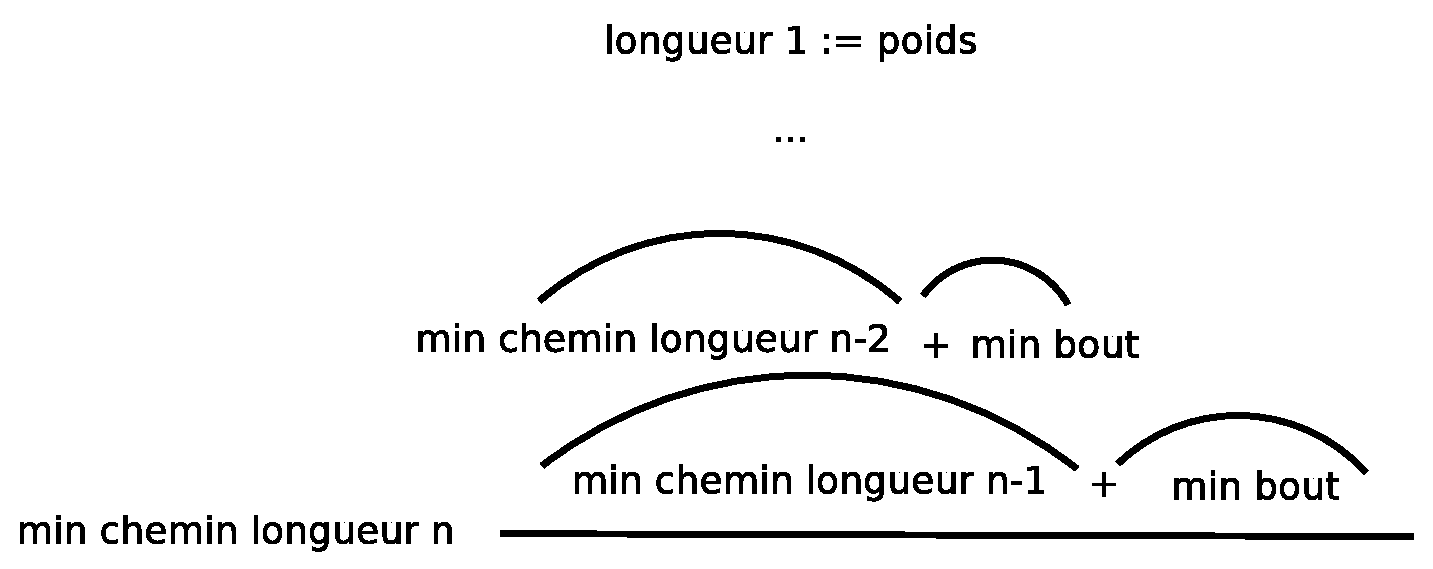
\includegraphics[height=5cm]{../images/tspDyn.eps}
\end{center}
\caption{Exemple de calcul d'un chemin pour le tsp en programmation dynamique.}
\end{figure}

\paragraph{Principe de l'algorithme}

Nous proposons l'algorithme suivant pour une programmation dynamique
du TSP.

\begin{algorithm}[!ht]
\caption{Programmation dynamique pour le TSP}
\label{Dyntsp}
\begin{algorithmic}[1]
\REQUIRE une matrice de poids, un ensemble de $n$ sommets
\FOR{chaque sous-ensemble $S$ commençant par $0$}
\IF{$|S| = 2$}
\FOR{$i$ de $0$ à $n-1$}
\STATE C[S][i] := poids[0][i]
\ENDFOR
\ELSE
\FOR{$i$ de $0$ à $n-1$}
\FOR{tous les $k$ $\notin$ $S - \{ 0 \}$}
\STATE C[S][i] := $\min$ $\{$ C[$S - \{ k \} $][k] + poids[k][i] $\}$
\ENDFOR
\ENDFOR
\ENDIF
\ENDFOR
\STATE retourner $\min$ $\{$ C[S][i] + poids[i][0] $\}$ avec $|S| = $
(nombre de sommets - 1)
\end{algorithmic}
\end{algorithm}

\paragraph{Complexité théorique}

La complexité théorique d'un tel algorithme est de $O(n^2.2^n)$.

\paragraph{Tests unitaires}

Comme déjà décrit auparavant, nous avons également mené différents
tests unitaires sur diverses instances du TSP. 


Exemple~:

\begin{lstlisting}
#define TSP_UNIT2_N_OBJ 5
#define TSP_UNIT2_DISTANCES {               \
                              {0,1,2,1,0},  \
                              {1,0,3,5,0},  \
                              {2,3,0,2,1},  \
                              {1,5,2,0,4},  \
                              {0,0,1,4,0}   \
                            }
#define TSP_UNIT2_RIGHT_ANSWER 5
\end{lstlisting}

\paragraph{Jeux de tests et temps d'exécution}
Nous mesurons ici une moyenne du temps d'exécution sur 5 tests en
faisant varier le nombre de sommets à parcourir. Nous obtenons les
résultats présentés ci-dessous.

\begin{table}[h!]
\centering
\begin{tabular}{|c|c|}
\hline
Sommets & temps d'exécution moyen en ms\\
\hline
2 & 0\\
\hline
5 & 2\\
\hline
7 & 15\\
\hline
9 & 137\\
\hline
11 & 1151\\
\hline
13 & 8575\\
\hline
15 & 58109\\
\hline
\end{tabular}
\caption {Variation du temps d'exécution en fonction du capacité du sac}
\end{table}


\begin{figure}[h!]
\centering
\begin{tikzpicture}[scale=1.2]
    \begin{axis}[title=Jeux de tests pour le TSP, xlabel= nombre de
        villes parcourues, ylabel= temps d'exécution]
      \addplot
        table[col sep=comma]{tspdyn.csv};
        \legend{exécution de sac à dos}
    \end{axis}
\end{tikzpicture}
\caption{Temps d'exécution du voyageur de commerce.}
\end{figure}

\paragraph{Conclusion sur la complexité}

\pagebreak

\subsection{Branch and bound}

Nous nous intéresserons au sein de cette section à la programmation de
la méthode de branch and bound pour résoudre le problème du voyageur
de commerce (tsp).

\subsubsection{Détermination de la solution initiale}

 Nous nous intéresserons à trois heuristiques en particulier.
\begin{itemize}
\item Chaîne de poids le plus faible et ajout d'une arête pour le
  cycle
\item Voisinage 2--opt
\item Voisinage 3--opt
\end{itemize}

\subsubsection{Principe de l'algorithme}

\paragraph{Algorithme}

Nous proposons d'implémenter l'algorithme récursif présenté ci-dessous.

\begin{algorithm}[!ht]
\caption{Branch and Bound pour le TSP}
\label{BBtsp}
\begin{algorithmic}[1]
\REQUIRE un sommet racine, une borne inférieure, un graphe $G$
\STATE faire ACPM $G - \{x \}$
\STATE relier $x$ à ses deux voisins les plus proches en terme de coût
\IF{valeur du cycle > borne inférieure}
\IF{tous les sommets sont de degré $2$}
\STATE mettre à jour le solution courante
\ELSE
\STATE choisir un sommet $y$ de degré $\geq$ 2
\FOR{chaque arête $e_i$ issue de $y$}
\STATE $G' := G - \{ e_i \}$
\STATE BranchAndBound($y$, borne inférieure, $G'$)
\ENDFOR
\ENDIF
\ENDIF
\STATE retourner la plus petite des solutions acceptables
\end{algorithmic}
\end{algorithm}

La borne inférieure est une solution initiale obtenue grâce à une heuristique.

\paragraph{Complexité théorique}

TODO

\subsubsection{Implémentation}

Nous n'avons pas pu mener de tests sur le branch and bound pour le tsp
suite à des erreurs de compilation non réglées à ce jour. Cependant,
nous avons tenté de proposer une implémentation de l'algorithme décrit plus haut
en Ocaml (à l'aide de la bibliothèque Graph Pack), dont voici un extrait~:
\begin{lstlisting}
let rec branchBound g x borneInf solution = 
	       let g' = copy g in
	       remove_vertex g x
	       let arbre = spanningtree g in
	       let cycle = relier x g' g in 
	       let val = valeurCycle cycle in
	       if val > borneInf then 
		 if tousDegre2 cycle then
		   solution = val
		 else
		   let y = choixSup2 g in
		   let aretesSucc = succ_e g y in 
		   let listeSolutions = map branche aretesSucc in
	       else()
		 solution = min listeSolutions
\end{lstlisting}

\subsection{Programmation de l'algorithme $\frac{3}{2}$}

\subsubsection{Principe de l'algorithme}

\paragraph{Algorithme}

L'algorithme $\frac{3}{2}$ que nous proposons est le suivant~:

\begin{algorithm}[!ht]
\caption{Approximation $\frac{3}{2}$ pour le TSP}
\label{3-2tsp}
\begin{algorithmic}[1]
\REQUIRE un graphe $G$
\STATE faire ACPM $T$ $G$ de coût $w$
\STATE $W := $ sommets de degré impair de $T$
\STATE chercher un couplage $M$ de $G$ poids min $m$ saturant tous les
sommets de $W$
\STATE $G' := $ le graphe construit à partir des arêtes de $M$ et de
$T$
\STATE Soit P un parcours eulérien de longueur $p$, on a $p:= w + m$
\STATE retourner un cycle de longueur $c \leq p$
\end{algorithmic}
\end{algorithm}

\paragraph{Complexité théorique}

TODO

\subsubsection{Implémentation}

Nous n'avons pas eu le temps d'implémenter cet algorithme. Néanmoins,
nous aurions probablement utilisé le langage C/C++ avec la
bibliothèque boost::graph pour cela. De plus, nous aurions mesuré les
temps d'exécution de nos fonctions à l'aide de l'outil de profiling gprof.

\section{Conclusion}

\end{document}
